\section{Software}
\subsection{As-is Implementation}
The as-is data processing pipeline of Pookie is illustrated in Figure \ref{fig:flow-as-is}. In summary, the robot accepts real time inputs in the form of image frames and sound from its camera and microphone, then passes it through the facial and speech emotion recognition models respectively. Next, given a timeframe (e.g every 5 seconds), the models select the dominant emotion (i.e emotions with the highest confidence) then decide on the next best action based on that. For instance, if the dominant emotion from the FER and SER side are happy, then the output would be positivity maintenance. 

\begin{figure}[ht]
    \centering
    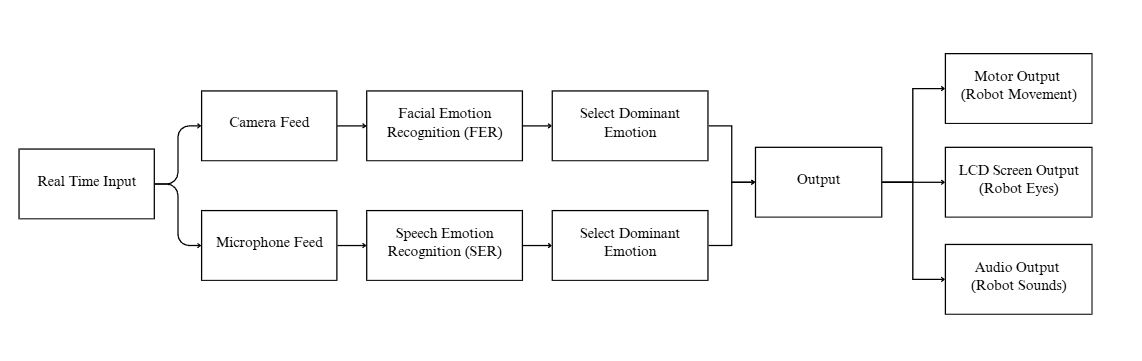
\includegraphics[width=\textwidth]{flow_as_is.png}
    \caption{Pookie As-is Implementation}
    \label{fig:flow-as-is}
\end{figure}

However, this design posed a few problems. Firstly, it does not take into consideration what the “true” emotion of the user is, which is fundamentally important. When people question what another person’s emotion is, they don’t look at the face and speech separately, but rather as one single emotion that captures what the person is feeling. We approached this problem by setting up a hypothesis of what the user could be feeling, then updating it with evidence from the FER and SER models, through using Bayesian Networks, which will be discussed in the next section. 

The next problem is ambiguity. Let’s say the output produced from FER and SER are 50\% happy and 50\% sad. With the initial approach, this case would be resolved using random selection, either sad or happy. However, this solution is quite ambiguous, and does not reflect realistic emotions. Thus, we decided to implement simplified decision trees, which use thresholds as a rule in navigating between nodes. The solution helps Pookie consistently navigate through complex or ambiguous emotions, but requires a lot of careful work in designing each node. This will be discussed in detail in the next section. 


\subsection{Challenges}
This section will discuss the challenges that were encountered during implementation. One major problem is the ambiguity of mapping of emotions. For context, each of the FER and SER emotions output a JSON of probabilities and their confidence (e.g Happiness 60\%, Neutral 30\%, Anger 10\%), with the potential outputs from each model shown in Table \ref{tab:emotion_mapping}. As shown in the figure, the models do not produce outputs with a 1:1 relationship, meaning some emotions from FER do not have a SER counterpart (such as FER output “Fear” does not have a corresponding emotion on the SER side). 

\begin{table}[h]
    \centering
    \begin{tabular}{|c|c|}
        \hline
        \textbf{Facial Emotion Recognition (FER) Outputs} & \textbf{Speech Emotion Recognition (SER) Outputs} \\
        \hline
        Neutral   & Neutral   \\
        \hline
        Anger     & Anger     \\
        \hline
        Happiness & Happiness \\
        \hline
        Sadness   & Sadness   \\
        \hline
        Disgust   & Frustration \\
        \hline
        Fear      & -         \\
        \hline
        Surprise  & -         \\
        \hline
    \end{tabular}
    \caption{Mapping of Emotions for SER and FER}
    \label{tab:emotion_mapping}
\end{table}

This inconsistency prevents the processing pipeline from functioning properly, necessitating the development of a solution. We have decided to map the missing speech emotion outputs to the most relevant existing speech emotions. While this approach may introduce some ambiguity, it provides a temporary fix for the emotion mapping issue. The newly mapped emotions are shown in Table \ref{tab:revised_mapping}.

\begin{table}[h]
    \centering
    \begin{tabular}{|c|c|}
        \hline
        \textbf{Facial Emotion Recognition (FER) Outputs} & \textbf{Speech Emotion Recognition (SER) Outputs} \\
        \hline
        Neutral   & Neutral   \\
        \hline
        Anger     & Anger     \\
        \hline
        Happiness & Happiness \\
        \hline
        Sadness   & Sadness   \\
        \hline
        Disgust   & Frustration \\
        \hline
        Fear      & Sadness (SER)   \\
        \hline
        Surprise  & Neutral (SER)   \\
        \hline
    \end{tabular}
    \caption{Revised Mapping of Emotions for SER and FER}
    \label{tab:revised_mapping}
\end{table}

In order to reduce the ambiguity caused by this substitution approach, we sought guidance from our advisor, Professor Paulo Garcia, who recommended exploring the Bayesian Network approach. The Bayesian Network approach will be discussed further in the next section.

\subsection{Revised Implementation using Bayesian Networks}

A Bayesian Network is a probabilistic graphical model that represents a set of variables and their conditional dependencies using a directed acyclic graph (DAG). It provides a structured approach to reasoning under uncertainty by encoding the probabilistic relationships between variables. In the context of Pookie, the Bayesian Network is used to infer the user's true emotional state by integrating evidence from both the FER and SER models.

The revised implementation introduces a Bayesian Network shown in Figure \ref{fig:bn}, where the user's underlying emotional state is treated as a latent variable, which is updated dynamically as new observations from FER and SER arrive. The network consists of nodes representing possible emotions and edges that define the probabilistic dependencies between them. Given an initial prior belief about the user's emotion, the system updates its belief by incorporating new observations from the FER and SER models using Bayes’ Theorem.

\begin{figure}[ht]
    \centering
    \includegraphics[width=\textwidth]{bn.png}
    \caption{Pookie's Bayesian Network}
    \label{fig:bn}
\end{figure}

\newpage
To construct the Bayesian Network, we defined conditional probability tables (CPTs) based on confusion matrices from both the FER and SER models seen in Figure \ref{fig:fer} and \ref{fig:ser} respectively, as well as insights from \textit{Emotions in Everyday Life} by Trampe et al. (2015) \cite{10.1371/journal.pone.0145450}, which provides probability distributions of emotions. By analyzing the confusion matrices, we estimated the likelihood of misclassifications and incorporated these probabilities into the CPTs, ensuring a more accurate representation of emotional relationships.

\begin{figure} [!ht]
    \centering
    \begin{minipage}{0.45\textwidth}
        \centering
        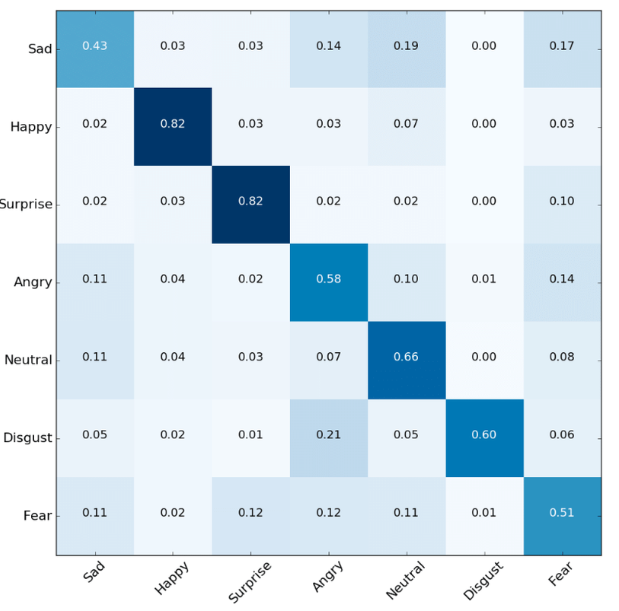
\includegraphics[width=\linewidth]{fer_confusion.png}
        \caption{FER Confusion Matrix}
        \label{fig:fer}
    \end{minipage}
    \hfill
    \begin{minipage}{0.45\textwidth}
        \centering
        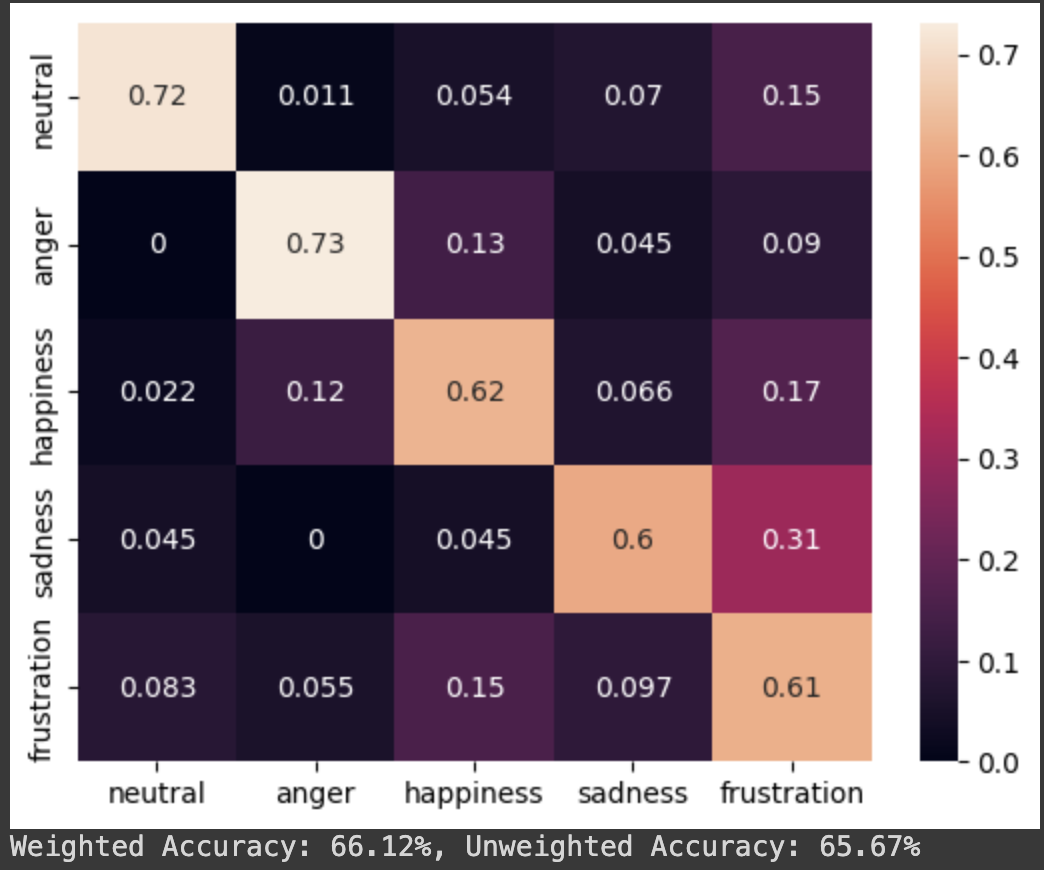
\includegraphics[width=\linewidth]{ser_confusion.png}
        \caption{SER Confusion Matrix}
        \label{fig:ser}
    \end{minipage}
\end{figure}

The confusion matrices represent how often the models correctly and incorrectly classify different emotional states. By utilizing these matrices, we were able to estimate the conditional probabilities for each emotional state. For example, if the FER model often misclassifies "Fear" as "Surprise" or "Sadness," these relationships are reflected in the CPTs. Similarly, if the SER model has a tendency to confuse "Frustration" with "Anger," the Bayesian Network accounts for these uncertainties when updating its belief about the user’s true emotion.

By combining the confusion matrix data with the probability distributions from the research paper, we constructed CPTs that better capture real-world emotional correlations. This approach allows the Bayesian Network to weigh the reliability of each model's predictions and adjust the estimated emotional state accordingly. Instead of treating FER and SER outputs as absolute truths, the system considers their likelihood of being correct based on historical performance.

To update the belief about the user’s emotional state, the Bayesian Network relies on Bayes’ Theorem, which provides a framework for calculating conditional probabilities. Specifically, the network uses the formula:

\[
P(E \mid R) = \frac{P(R \mid E) \cdot P(E)}{P(R)}
\]

Where:
\begin{itemize}
    \item \( P(E \mid R) \) is the posterior probability, representing the probability of the emotional state \( E \) given the result \( R \) (i.e., the FER and SER outputs).
    \item \( P(R \mid E) \) is the likelihood, which indicates how likely the result \( R \) is, given the emotional state \( E \).
    \item \( P(E) \) is the prior probability, representing the initial belief about the emotional state before observing the result, which is informed by the emotion distribution provided in \textit{Emotions in Everyday Life} by Trampe et al. (2015) \cite{10.1371/journal.pone.0145450}.
    \item \( P(R) \) is the evidence, or the total probability of observing the result under all possible emotional states.
\end{itemize}

In the context of Pookie, the emotional state \( E \) could be one of the possible emotions such as happiness, sadness, anger, etc. The result \( R \) is derived from the outputs of the FER and SER models, which provide a set of probabilities for each emotion. The likelihood \( P(R \mid E) \) is determined by the confusion matrices of the FER and SER models, which reflect how likely it is for the models to generate certain outputs given the true emotional state.

In this case, the likelihood \( P(R \mid E) \) is represented as the product of the probabilities from both the Facial Emotion Recognition (FER) and Speech Emotion Recognition (SER) models. Since we are dealing with two different models that provide independent estimates of the user’s emotional state, we combine these estimates by multiplying their corresponding probabilities for each emotion.

Thus, the likelihood for each possible emotional state \( E \) given the result \( R \) (which consists of the outputs from both the FER and SER models) can be expressed as:

\[
P(R \mid E) = P(R_{\text{FER}} \mid E) \cdot P(R_{\text{SER}} \mid E)
\]

Where:
\begin{itemize}
    \item \( P(R_{\text{FER}} \mid E) \) is the probability of the FER result \( R_{\text{FER}} \) given the emotional state \( E \).
    \item \( P(R_{\text{SER}} \mid E) \) is the probability of the SER result \( R_{\text{SER}} \) given the emotional state \( E \).
\end{itemize}

Since the FER and SER models are independent, their combined likelihood is simply the product of their individual likelihoods. This approach assumes that facial and speech expressions are conditionally independent given the true emotional state. By multiplying the probabilities, we take into account both the visual and auditory evidence of the user’s emotion, and use the combined evidence to estimate the true emotional state more accurately.

Thus, the updated Bayesian formula for computing the posterior probability of the emotional state \( E \) given the observations \( R_{\text{FER}} \) and \( R_{\text{SER}} \) becomes:

\[
P(E \mid R_{\text{FER}}, R_{\text{SER}}) = \frac{P(R_{\text{FER}} \mid E) \cdot P(R_{\text{SER}} \mid E) \cdot P(E)}{P(R_{\text{FER}}, R_{\text{SER}})}
\]

Where:
\begin{itemize}
    \item \( P(R_{\text{FER}}, R_{\text{SER}}) \) is the evidence or the total probability of observing both the FER and SER results. This is computed as the sum of the likelihoods over all possible emotional states:
\end{itemize}

\[
P(R_{\text{FER}}, R_{\text{SER}}) = \sum_{E} P(R_{\text{FER}} \mid E) \cdot P(R_{\text{SER}} \mid E) \cdot P(E)
\]

This formulation ensures that the system updates its belief about the user's emotional state by considering the likelihood of both the FER and SER outputs for each possible emotion. By combining the results from the facial and speech emotion recognition models, the Bayesian Network effectively integrates multiple sources of evidence, resulting in a more robust and accurate estimate of the user's true emotional state.

The use of multiplication for the likelihoods allows the Bayesian Network to properly account for the evidence from both modalities, reducing the impact of uncertainties and ambiguities from individual models. This approach improves the overall accuracy of the emotional assessment and enhances the robot's ability to make decisions that align with the user's true feelings.

The prior \( P(E) \) is based on a generalized distribution of emotional states, derived from external research, such as the findings from \cite{10.1371/journal.pone.0145450}. It reflects the average emotional distribution across a population and does not adjust based on an individual user’s history or context. This prior probability serves as a baseline, representing the general likelihood of each emotional state before any new observations from the FER and SER models are made.

Finally, \( P(R) \), the evidence, ensures that the posterior probabilities of all possible emotional states sum to 1. This value can be calculated as the sum of the likelihoods over all possible emotional states:

\[
P(R) = \sum_{E} P(R \mid E) \cdot P(E)
\]

By applying Bayes’ Theorem iteratively as new observations from the FER and SER models arrive, the Bayesian Network updates its belief about the user's emotional state. This update does not involve refining the estimate based on previous emotional history, but rather adjusts the system’s estimate by integrating the evidence from the two models in real time. This process allows the system to more accurately infer the user’s emotional state and navigate complex emotional situations with greater precision, reducing ambiguity and improving the overall user experience.

This probabilistic model enables Pookie to move beyond simple rule-based decision-making and handle the complexity of real-world emotional states more effectively.
